\documentclass[letterpaper]{article}

% authors and affiliations
\title{PMoveSTIR---A general framework to incorporate movement and space use information in epidemiological models}
\usepackage{authblk}
\author{Juan S. Vargas Soto \and Mark Q. Wilber}
\affil{School of Natural Resources, University of Tennessee, Knoxville, TN}
\date{}


\usepackage[english]{babel}
\usepackage[utf8x]{inputenc}
\usepackage{amsmath}
\usepackage{graphicx}
\usepackage[left=1 in, right=1 in, top=1 in, bottom=1 in]{geometry}
% \usepackage{hyperref}
\usepackage{bbold}
\usepackage{rotating}
\usepackage{bbm}
\usepackage{array}
\newcolumntype{C}[1]{>{\centering\arraybackslash}m{#1}}
% \usepackage{kbordermatrix}
\usepackage{footnote}
\makesavenoteenv{tabular}
\makesavenoteenv{table}
% \renewcommand{\theequation}{{S}\arabic{equation}}

\makeatletter
% \addto\captionsenglish{%
%   \renewcommand{\fnum@figure}{Figure S\thefigure}%
%   \renewcommand{\fnum@table}{Table S\thetable}%
% }
\makeatother

% Bibliography
\usepackage[round, colon]{natbib} % Bibliography - APA
\bibliographystyle{abbrvnat}
%\bibpunct{(}{)}{;}{a}{}{,}

% Line numbers
\usepackage{lineno}
%\def\linenumberfont{\normalfont\footnotesize\ttfamily}
%\setlength\linenumbersep{0.2 in}
\linenumbers

% Set space
\usepackage{setspace}
\doublespacing

% Command to e.g. write code that doesn't show up. Used as \ignore {some code}
\newcommand{\ignore}[1]{}

\begin{document}

\maketitle

\section*{Introduction}

Individual movement is among the most critical factors that determine spatial dynamics of infectious disease in wildlife \citep{Manlove2022,Dougherty2022}. 
For example, the combined dispersal of individuals in a population defines how parasites and infectious diseases spread across the landscape \citep{Fofana2017}. 
At a more local scale, how an animal moves determines whether they encounter other individuals of the same species, other species, or parasites in the environment. 
These encounters are a necessary component for parasite transmission, and efforts have sought to identify where they could occur, how often, and more importantly, how they are influenced by environmental drivers.  
Being able to formally link environmental factors, animal movement, contact, and parasite transmission risk, could improve our ability to predict and prevent outbreaks and would represent a significant advancement for management of wildlife diseases. 
Nevertheless, understanding and extrapolating the relationships between these processes remains an outstanding task in disease ecology \citep{White2018}.

Technological and analytical advances in movement ecology now provide unparalleled insight into the links between animals and their environment. 
From tracking data we can characterize the way animals move \citep{Abrahms2017}, infer their behavioral state \citep{Langrock2012}, determine how their movement is influenced by the environment \citep{Avgar2015,Potts2022}, or how it is modified through interactions among individuals \citep{Scharf2016, Scharf2018}. 
The high spatial and temporal resolution of modern tracking data also serves to create biologically realistic movement models, and from those to estimate detailed utilization distributions (UDs) \citep{Fleming2014,Gurarie2011,Potts2023}.
An individual's UD is defined as the probability--either transient or in the long-run (Tao)--that it uses a particular area on a landscape, and is perhaps the best representation of the relationship between space and animal movement. 
%UDs are an esential tool for linking animal movement and transmission, because of their wide-spread use, intuitive understanding, and biological underpinnings.
UDs are defined at the individual level but they are particularly useful to study the interaction between individuals, for example to quantify the overlap between home ranges, or to estimate where two animals are most likely to encounter each other \citep{Noonan2021}, both of which can have important implications for disease transmission. 
Moreover, because UDs can be directly linked to environmental drivers of movement \citep{Signer2017}, they have the potential to predict contact and transmission in novel environments and can also be used for prospective analyses to understand how the effects of environmental and social perturbations cascade across scales, from individual movement to population and landscape-level disease transmission. 
Some studies have used metrics such as home range overlap to build contact networks \citep{Godfrey2010, Godfrey2013}, yet only recently have studies formally linked UDs with animal contacts.


%To understand how movement impacts epidemiological dynamics, we first need to properly characterize movement and how it relates to space and resource use. 
%This is a challenging task, because movement is the product of a complex interplay between physiology, resource availability and distribution, landscape features, and inter- and intraspecific interactions \citep{Nathan2008,Merkle2018,Vanderwaal2017}, and it can be hard to disentangle their influence.
%Similarly, we can use fine-scale spatiotemporal data to infer where and when contact between animals occurs \citep{Noonan2021}, and to build contact networks for direct \citep{Craft2015} and indirect interactions \citep{Yang2023}. 
%There has been less work dedicated to linking landscape with parasite transmission \citep{Merkle2018,Tracey2014}.

%The utilization distribution (UD) plays a central role in linking host movement to contact and transmission, and could be a key to link these processes with environmental drivers. 
%UDs can be derived directly from spatial and social factors driving movements and continuous-time movement models can be used to calculate biologically realistic utilization distributions \citep{Potts2023}[Potts citation, Flemming citation]. 

One such approach developed by \citet{Noonan2021} showed how UDs could be used to predict the conditional distribution of encounters (CDE) between pairs of individuals, i.e. the probability that two individuals will come into contact with each other at a given location.
This work is an important advance in linking empirical movement to contact, but two key challenges remain to move from UDs to predictions of disease transmission.  
First, the CDE estimator assumes that movement is independent between individuals.
While a useful simplification, social interactions can invalidate this assumption and may play a significant role in transmission dynamics \citep{Manlove2018} [another citation]. For example, territorial animals avoid each other not only in space, also in time \citep{Giuggioli2013}, such that even territorial animals with some spatial overlap may rarely come into direct contact.  In gregarious species, the trajectories of individuals within a group overlap substantially in space and time. Similarly, pairs of some solitary species travel together for short periods during courtship or nursing, but otherwise move independently. In all these cases, temporal correlations (positive or negative) in space use could increase or decrease the expected probability of encounter compared to an assumption of independent movement. In general, we lack a way to quantify the role of social interactions on spatio-temporal force of infection, which limits our ability to assess whether ignoring correlated movements actually matters when assessing infection risk. One of our goals in this study is to ask: how much can correlated, social movements affect spatio-temporal infection risk?

%These could have implications for epidemiological contact, but their effect is not captured by the CDE estimator based on stationary UDs. 

The second challenge is that while the CDE describes direct contact, it does not fully capture epidemiological contact consisting of contact formation, contact duration, pathogen acquisition, pathogen shedding, and pathogen decay. Pathogen decay is particularly important when accounting for indirect contacts where transmission can happen when individuals are in the same place but at different times \citep{Wilber2022,Yang2023,Richardson2015}.  As some parasites can persist in the environment for months or years (anthrax, CWD), indirect transmission can contribute substantially restrucure transmission risk compared to direct transmission alone \citep{Yang2023}.  Moreover, the CDE is expressed as a normalized probability density per unit area, whereas an epidemiological contact would ideally be described as a force of infection, with units per time or per area per time.  When contact is direct and hosts move independently, this is largely a matter of standardizing and scaling the CDE estimate appropriately, but being explicit on how this scaling is achieved is crucial for linking UDs to predictions of disease spread.

Recent approaches developed at the interface of movement and contact ecology address some of these challenges \citep{Wilber2022,Yang2023}. For example, movement-driven modeling of spatio-temporal infection risk (MoveSTIR) builds dynamic spatio-temporal contact networks using realized movement trajectories. While MoveSTIR implicitly accounts for correlation among animals when building contact networks, it is an approach based on occurrence distributions \citep{Alston2022} -- i.e. it only considers where animals were observed moving and not where they potentially could have moved. Thus, in contrast to the CDE which is build around UDs \citep[a range-distribution method in the terminology of][]{Alston2022}, MoveSTIR is not as well-suited for predicting how social or environmental changes affect UDs and thus affect contact and transmission.  On the other hand, MoveSTIR provides general theory to translate contacts into the epidemiological currency of force of infection. Ultimately, an approach is needed that combines the range-distribution inference of UDs and CDEs \citep{Alston2022,Noonan2021} with the epidemiological focus of MoveSTIR to link UDs to epidemiological dynamics. 

Here, we develop a model we refer to as probabilistic MoveSTIR (PMoveSTIR) to estimate epidemiological contact and force of infection across space time from utilization distributions. In contrast to MoveSTIR which focuses on deriving epidemiological inference from fine-scale movement data and \emph{occurrence} distributions, PMoveSTIR derives epidemiological risk from \emph{range} distributions, of which UDs are a general case \citep{Alston2022}.  This has the advantage of providing probabilistic, spatio-temporal contact networks that can be used to predict out-of-sample transmission risk under independent or correlated movements. We first derive the most general PMoveSTIR model using transient UDs and then show how under assumptions of statistical stationarity and and independent movements PMoveSTIR is proportional to the CDE (but represents transmission risk in the units of force of infection). We also show how PMoveSTIR encompasses other common assumptions such as mass action transmission and home range overlap transmission as special cases.  Using PMoveSTIR and simulate movement data, we demonstrate the sometimes sizable importance of non-independent movements on pairwise transmission risk, indicating that ignoring the social drivers of contact could severely bias epidemiological inference.  We demonstrate the importance of this result in a real dataset on white-tail deer movements where we show that correlated movements can increase potential force of infection by orders of magnitude [Adjust as necessary].  Overall, PMoveSTIR is a critical next step for developing predictive models that link movement data to spatio-temporal infection dynamics on real landscapes.

% Moreover.   Using MoveSTIR
% Our work is an extension of the MoveSTIR framework developed by \citet{Wilber2022}. 
% MoveSTIR provides a generalizable model for leveraging spatially and temporally explicit movement data to understand epidemiological dynamics. The theoretical framework should also be flexible enough to use different types of data like GPS collars, proximity loggers, or camera-traps \citep{Wilber2022}. 
% This framework is defined explicitly in terms of epidemiological processes, allowing to tease apart individual contributions to the overall transmission across the population, to other specific individuals, or to specific locations. 
% MoveSTIR relies exclusively on \emph{observed} data, for example as could be obtained form GPS-tracking devices. Instead, we adopt a probabilistic approach, to estimate an expected force of infection across space and time. 
% Putting the moveSTIR transmission kernel in a similar framework to existing methods of movement analysis could facilitate linking mechanistically environmental variables with the transmission process. 
% We start by developing the theoretical framework for the general and special cases. Then, we use simulated data to explore the implications of our approach. Finally, we use an empirical data example with white-tailed deer to analyze the 
%Calculating the full transmission kernel can be computationally costly, and this cost increases with finer temporal resolution—observed or interpolated, with more individuals, and with longer tracking time. Depending on the study system, a more general approach with simplifying assumptions could capture the epidemiological dynamics in a similar way. 

% <!--# This language is very vague right now, need to fix and clarify -->
%Here, we generalize the moveSTIR model for multiple scenarios. Our goal is to develop a common framework that captures a majority of study cases related to wildlife movement and disease transmission, and that can make use of different data streams (e.g. GPS tracking, proximity/contact loggers, camera-traps).

% While considering only direct contacts is likely sufficient for many ecological processes, indirect interactions cannot be overlooked in the context of disease transmission. 
% Many parasites can persist in the environment--for months or years in some cases--and be transmitted without direct contact between hosts. 
% Ignoring indirect contacts can drastically reshape disease transmission networks and the inferences about epidemiological dynamics \citep{Wilber2022,Yang2023,Richardson2015}.


%% Juan: Not  sure how much of an issue this is, if we only consider only direct transmission getting an FOI-like term is just a matter of standardizing and scaling. I think the real issue is the assumption of independence and the correlation, which are related. 

%Thus, it is unclear how ignoring the temporal correlation component would affect inferences about epidemiological processes. 

%% some thoughts: 
% 1.What we have developed, at least the component in brackets, is a different estimator of the CDE, that actually considers correlation across individuals. I think this is an interesting development not just for transmission but for encounter theory in general. 
% 2. I think all the limitations are one and the same, simply that Noonan's estimator ignores temporal correlation. 



\section*{Methods}

\subsection*{Linking utilization distributions to transmission through PMoveSTIR}

Consider two individuals, $i$ and $j$, moving and interacting across a landscape.  We want to ask: on average across space and time what is the potential or realized force of infection (FOI) host $i$ feels from host $j$ in some location $x$?  The FOI is an essential quantity to estimate in disease ecology that underlies our ability to predict the spread of disease across populations and landscapes. Here we develop the approach PMoveSTIR that formally links host utilization distributions, direct and indirect contacts, and spatial estimates of force of infection.

PMoveSTIR builds on the recently developed MoveSTIR model. In MoveSTIR and PMoveSTIR we assume that transmission happens by one host depositing pathogen into the environment and another host picking that pathogen up.  Deposition and acquisition can represent a range of processes, from one individual coughing and another inhaling in a matter of seconds to one host depositing parasite eggs in the environment and another individual consuming these eggs days or weeks later. This fairly general assumption encompasses standard density-dependent transmission as a special case \citep{Cortez2021}. Moreover, considering transmission through deposition and acquisition components clearly links direct transmission and indirect transmission along a continuum \citep{Wilber2022}.

Given these transmission assumptions, we can define the pairwise force of infection felt by host $i$ in location $x$ from host $j$ at time $t$ as \citep{Wilber2022}
\begin{equation}
    h_{i \leftarrow j}(t, x) = \int_{-\infty}^{t} \beta' \lambda \delta_{x_j(u)}(x) \delta_{I_j(u)}(I) S(t - u) du
    \label{eq:original_foi}
\end{equation}
<<<<<<< HEAD
where $\beta'$ is the pathogen acquisition rate of host $i$, $\lambda$ is the pathogen deposition rate of host $j$, $\delta_{x_j(u)}(x)$ is an indicator variable that is one if host $j$ is in location $x$ at time $u$ and zero otherwise, $\delta_{I_j(u)}(I)$ is an indicator function that is one if host $j$ is in an infected state at time $u$ and zero otherwise, and $e^{-\nu(t - u)}$ is the probability that any pathogen deposited at time $u < t$ is still alive at time $t$ \citep[see][for a full derivation]{Wilber2022}.  Moving forward we will make an assumption of maximum transmission risk and assume that host $j$ is always infected. This is equivalent to building a contact network and also represents the structural form of FOI needed to compute pathogen invasion thresholds \citep{Wilber2022}.

%It is beneficial to pause and consider the interpretation of ``contact'' and the parameter $\beta'$.  
We interpret that a ``contact'' can occur when both individuals visit a given location $x$. This could be a habitat patch or a grid cell, such that contact can only occur when two hosts are within the same habitat patch or grid cell. 
% IMPORTANT: There could be some mention here of the threshold distance. The interpretation as habitat patch may not be adequate if the patch is much larger than the threshold distance.
Importantly, we assume that locations $x$ on the landscape do not overlap such that summing locations $x$ equals some total area over which individuals can move (see SI for a derivation when $x$ is a point, not an area, on the landscape). Furthermore, we assume that the likelihood of contact is uniform within the location $x$, consistent with a so-called top hat encounter function \citep{Gurarie2013,Wilber2022}.

The term $\beta'$ is the rate at which host $i$ picks up pathogen within the location $x$ and can be re-written as $\tilde{\beta} / A_x$, where $\tilde{\beta}$ has units area / time (e.g., $m^2 / \text{day}$) and $A_x$ gives the area of location $x$ (e.g., 10 $m^2$). Therefore, the total acquisition rate scales with the area in which contact can occur. Larger areas would mean that host $i$ has to search for longer to find a ``packet'' of pathogen deposited by $j$, reducing $i$'s total acquisition rate and the corresponding force of infection.
%The same amount of pathogen spread over a larger area would reduce the total acquisition rate .  deposited by host $j$  (or, equivalently, host $i$ would have to traverse a larger area ),  .  
As we derive PMoveSTIR, it is critical to be specific about our definition of contact and the area units associated with $\beta'$.  

Considering probabilistic movements, we can re-write equation \ref{eq:original_foi} as

\begin{equation}
    h_{i \leftarrow j}(t, x) = \int_{-\infty}^{t} \beta' \lambda \delta'_{x_i(t)}(x) \delta'_{x_j(u)}(x) S(t - u) du
    \label{eq:prob_foi}
\end{equation}
where $\delta'_{x_i(\tau)}(x)$ and $\delta'_{x_j(\tau)}(x)$ are random variables that specify whether or not (i.e., 0 or 1) host $i$ or host $j$ is in location $x$ at time $\tau$ (e.g., in a grid cell).  This means that $h_{i \leftarrow j}(t, x)$ is also a random variable. Taking the expectation of $h_{i \leftarrow j}(t, x)$ with respect to repeated, hypothetical simulations of animal movement we obtain

\begin{equation}
    E[h_{i \leftarrow j}(t, x)] := h^*_{i \leftarrow j}(t, x) = \int_{-\infty}^{t} \beta' \lambda E[\delta'_{x_i(t)}(x) \delta'_{x_j(u)}(x)] S(t - u) du.
    \label{eq:expected_foi}
\end{equation}

Interpreting this expectation, we are asking: if we simulated some movement process thousands of times, what is the probability that host $i$ is in location $x$ at time $t$ and host $j$ was in location $x$ at a previous time $u$? 

\subsection*{Linking equation \ref{eq:expected_foi} to utilization distributions}

Our goal is to understand how utilization distributions link to spatio-temporal transmission risk.  To do that, first note that if $Y$ and $Z$ are two random variables, then $E[YZ] = E[Y]E[Z] + Cov(Y, Z)$.  We can therefore write equation \ref{eq:expected_foi} as

\begin{equation}
    \begin{aligned}
        h^*_{i \leftarrow j}(t, x) &= \int_{-\infty}^{t} \frac{\tilde{\beta}}{A_x} \lambda E[\delta'_{x_i(t)}(x) \delta'_{x_j(u)}(x)] S(t - u) du \\
        &= \frac{\tilde{\beta}}{A_x} \lambda \int_{-\infty}^{t} [E[\delta'_{x_i(t)}(x)] E[\delta'_{x_j(u)}(x)] + Cov(\delta'_{x_i(t)}(x), \delta'_{x_j(u)}(x))] S(t - u) du \\
        &= \frac{\tilde{\beta}}{A_x} \lambda \int_{-\infty}^{t} [p_i(x, t) p_j(x, u) + Cov(\delta'_{x_i(t)}(x), \delta'_{x_j(u)}(x))] S(t - u) du \\
    \end{aligned}
    \label{eq:foi_cov}
\end{equation}
where we use the fact that the expectation of an indicator variable is a probability \citep{Grimmett2001}. The terms $p_i(x, t)$ and $p_j(x, t)$ give the probabilities that host $i$ and $j$ are in location $x$ as time $t$ and can also be written as $p_i(x, t) = \int_{A_x} f_i(s, t) ds$ where $f_i(s, t)$ is the probability density of host $i$ using the point $s$ at time $t$ and integral is over the area $A_x$ (defined equivalently for host $j$). Thus, $f_i(s, t)$ and $f_j(s, u)$ are the transient utilization distributions of host $i$ and host $j$ and equation \ref{eq:foi_cov} shows how they relate to spatio-temporal FOI.

% Second, we could write equation \ref{eq:expected_foi} as 

% \begin{equation}
%     \begin{aligned}
%     h^*_{i \leftarrow j}(t, x) &= \int_{-\infty}^{t} \beta' \lambda E[\delta'_{x_i(t)}(x) \delta'_{x_j(u)}(x)] e^{-\nu(t - u)} du \\
%     &= \beta' \lambda \int_{-\infty}^{t} p(i \in x \text{ at } t, j \in x \text{ at } u) e^{-\nu(t - u)} du) \\
%     &= \beta' \lambda \int_{-\infty}^{t} p(i \in x \text{ at } t | j \in x \text{ at } u) p(j \in x \text{ at } u) e^{-\nu(t - u)} du \\
%     \end{aligned}
%     \label{eq:foi_prob}
% \end{equation}

To better understand the meaning of equation \ref{eq:foi_cov}, consider the special case of statistical stationarity in movement (i.e., the mean location are constant through time, though animal is still moving).  For clarity, also assume that pathogen survival in the environment follows $S(t - u) = e^{-\nu (t - u)}$, where $\nu$ is the pathogen decay rate.  We  can simplify equation \ref{eq:foi_cov} to (derivation in SI)

\begin{equation}
    \begin{aligned}
    E[h_{i \leftarrow j}(x)] = \frac{\tilde{\beta}}{A_x} \lambda [p_i(x)p_j(x) \frac{1}{\nu} + \int_{0}^{\infty} Cov(\delta_{i \in x}, \delta_{j \in x} | \tau) e^{-\nu \tau} d\tau]
    \end{aligned}
    \label{eq:foi_stationary}
\end{equation}
The key insight here is that, given a stationary assumption, the expected force of infection in location $x$ depends on i) the marginal probabilities that host $i$ and host $j$ use location $x$, where $p_i(x) = \int_{A_x} f_i(s) ds$ and $p_j(x) = \int_{A_x} f_j(s) d$ and $f_i$ and $f_j$ are the utilization distributions of host $i$ and $j$ and ii) the covariance in how host $i$ and host $j$ use location $x$ at different time lags $\tau$. For example, if host $i$ and $j$ always use location $x$ together (a positive correlation at time lag $\tau = 0$), this will increase the force of infection relative to the product of their utilization distributions.  

To gain some intuition into equation \ref{eq:foi_stationary}, consider the case of two hosts moving independently across a landscape.  Because hosts are moving independently, the covariance is zero such that $\frac{\tilde{\beta}}{A_x} \frac{\lambda}{\nu} p_i(x)p_j(x)$ -- the expected FOI experienced by two hosts is exactly proportional to the products of their utilization distributions \citep[similar to the result given in][]{Noonan2021}.  In this particular case the FOI is symmetrical, i.e. the FOI from $i$ to $j$ is the same as from $j$ to $i$.

Now assume hosts are moving independently and use space uniformly on a gridded landscape and contact occurs when individuals are in the same grid cell.  The area of grid cell $x$ is $A_x$ and the total area of the landscape is $A_{tot} = n A_x$, where $n$ is the number of grid cells that comprise $A_{tot}$. Because movement is random with respect to location, $p_i(x) = p_j(x) = \frac{A_x}{A_{tot}}$ and the force of infection at location $x$ is $\frac{\tilde{\beta}}{A_{tot}} \frac{\lambda}{\nu} \frac{A_x}{A_{tot}}$.  Finally, if we want the expected FOI from $j$ to $i$ over all space, we sum over all grid cells and get $\frac{\tilde{\beta}}{A_{tot}} \frac{\lambda}{\nu}$. This is exactly equivalent to the FOI we would expect using a mass action assumption of hosts moving independently and transmitting within an area $A_{tot}$ \citep{McCallum2001}.

% Instead of assuming hosts are moving uniformly across all $n$ grid cells, assume that they only occupy one grid cell on the landscape.  Now $p_i(x) = p_j(x) = 1$ if $x$ is the grid cell they use and is zero otherwise.  Applying the same steps and summing over all space we get $\frac{\tilde{\beta}}{A_{x}} \frac{\lambda}{\nu}$ -- the FOI from $j$ to $i$ is what we would expect if hosts were moving uniformly over a smaller area $A_x$. 

\subsection*{Applying equation \ref{eq:foi_cov} under different degrees of spatial and temporal heterogeneity}

Equation \ref{eq:foi_cov} is the most general formulation of PMoveSTIR. However, as we did in our example of statistically stationary movement above, it is useful to consider different degrees of spatial and temporal heterogeneity and how they simplify/modify equation \ref{eq:foi_cov}. This allows us to link different metrics such as temporally varying utilization distributions, stationary utilization distributions, and home range overlap to force of infection. In Fig. 1, we show how PMoveSTIR provides a general approach for accounting for different degrees of spatial and temporal heterogeneity in movement.

\subsubsection*{The upper right-hand corner: Heterogeneous space and time}

The upper right-hand corner is the most general case captured by equation \ref{eq:foi_cov} -- utilization distributions and between-individual spatial covariance are time-varying and heterogeneous in space.  For example, this general case accounts for daily changes in habitat use and social interactions. 

\subsubsection*{The lower right-hand corner: Heterogeneous space and stationary time}

In the lower-right corner of Fig. 1, we assume stationarity in time, but continue to allow heterogeneity in space, obtaining equation \ref{eq:foi_stationary} discussed above.  To improve intuition, we can redefine $Cov(\delta_{i \in x}, \delta_{j \in x} | s) = \sigma_i(x) \sigma_j(x) Cor(\delta_{i \in x}, \delta_{j \in x} | s)$, where $\sigma_i(x) = \sqrt{p_i(x)(1 - p_i(x))}$  and $\sigma_j(x) = \sqrt{p_j(x)(1 - p_j(x))}$ are the standard deviation in probability of host $i$ and $j$ using location $x$, respectively.  We can then write

\begin{equation}
    \begin{aligned}
    h^*_{i \leftarrow j}(x) = \beta' \lambda \left[ p_i(x)p_j(x) \frac{1}{\nu} + \sigma_i(x) \sigma_j(x) \int_{0}^{\infty} Cor(\delta_{i \in x}, \delta_{j \in x} | s) e^{-\nu s} ds\right].
    \end{aligned}
    \label{eq:stationary_cor}
\end{equation}
Equation \ref{eq:stationary_cor} highlights that the key quantity we need to understand is the correlation in host $i$'s and host $j$'s use of location $x$ at different time lags $s$. The correlation is most easily understood for short time lags ($s\approx0$); a positive correlation indicates that individuals are usually together, while a negative correlation indicates they rarely are. At longer time lags, the correlation indicates whether an individual avoids (negative correlation) or is attracted to (positive) a site following the passage of another individual. For example, a strong positive correlation at a short time lag when host $j$ lags $i$ but no correlation when host $i$ lags host $j$ would indicate that host $j$ is following host $i$. 

Given the scaling effect of parasite decay---captured in the term $e^{-\nu s}$---the effect of the correlation on the FOI is highest for short time lags and decreases with longer lags. Thus, the importance of correlated movements will depend on the biology of the parasite: for parasites that can persist long times in the environment such as anthrax and chronic wasting disease, correlation in host movements may significantly augment transmission risk compared to an assumption of no correlation.

% [MOVE TO DISCUSSION?] Given an assumption of stationarity, the correlation term must be strictly related to social interactions.  Any use of $x$ because of environmental resources is picked up by $p_i(x)$ or $p_j(x)$, and the correlation term is specifically capturing whether hosts are using location $x$ synchronously (positive correlation) or asynchronously (negative correlation) more than we would expect by chance.  This is useful because it clearly highlights how social processes can alter the predictions of contact relative to only the overlap of utilization distributions (Anni's stuff) -- synchronous habitat use would increase the FOI, while asynchronous use would decrease it. However, it is important to note that the additive terms in equation \ref{eq:stationary_cor} are not a perfect separation of spatial and social drivers of contact. If social factors are driving co-location they will also be present in determining $p_i(x)$ and $p_j(x)$. Thus, the marginal utilization distributions contain the effects of both spatial and social factors, but the correlation term is strictly related to social factors.  If the correlation is zero, then hosts are moving independently and $p_i(x)$ and $p_j(x)$ only reflect spatial factors.

\subsubsection*{The lower left-hand corner: Uniform space and stationary time}

In the lower left-hand corner of the PMoveSTIR framework (Fig. 1), we have the special case where space use is uniform and time is stationary. Given these assumptions, we can write the FOI equation as

\begin{equation}
    \begin{aligned}
        h^*_{i \leftarrow j}(A_x) = \beta' \lambda \left[\frac{A_x}{A_{tot}}\frac{A_x}{A_{tot}} \frac{1}{\nu} + \sigma_i(x) \sigma_j(x) \int_{0}^{\infty} Cor(\delta_{i \in A_x}, \delta_{j \in A_x} | s) e^{-\nu s} ds\right]
    \end{aligned}
    \label{eq:uniform_stationary1}
\end{equation}
where the correlation in contact is constant across all areas $A_x$ on the landscape (such that $\delta_{i \in A_x}$ indicates the use of some arbitrary area $A_x$).  

If hosts are moving independently (i.e., correlation is 0) we obtain $\frac{\tilde{\beta}}{A_x} \frac{A_x}{A_{tot}} \frac{A_x}{A_{tot}}  \frac{\lambda}{\nu}$. Given a gridded landscape with non-overlapping grids and $x$ is a single grid cell, summing over all $n$ areas $A_x$ that comprise the landscape yields $\bar{h}_{i \leftarrow j} =\frac{\tilde{\beta}}{A_\text{tot}} \frac{\lambda}{\nu}$, which is the standard mass action assumption.  However, note that when movement between individuals is correlated, the FOI predicted by mass action can either overestimate or underestimate the true FOI. 


\subsubsection*{The upper left-hand corner: Uniform space and heterogeneous time}

Another special case of PMoveSTIR is when space use is uniform, but movement is non-stationary.  In this case, it is not important where an individual is, just when. Considering this framing from an empirical point of view, proximity loggers deployed on individual hosts---a commonly used tool to measure among-animal contacts---only tell us when contacts between individuals occur, but not where.  Thus, we cannot make inference about spatial factors driving contacts, but can make inference on temporal processes.  We consider this case in a future study.

\subsection*{Beyond the corners of PMoveSTIR}

PMoveSTIR also accounts for other useful cases regarding how heterogeneity in space and time relate to the expected FOI host $i$ feels from host $j$.  We give two examples below.

\subsubsection*{Home range overlap}

A commonly used assumption for the edge weight between host $i$ and host $j$ is that it is proportional to home range overlap.  Home range overlap is an intermediate case of of PMoveSTIR (Fig. 1), where time is stationary and space use is uniform within a home range, and the area of contact is the home range overlap.  Given that the area of home range overlap between host $i$ and host $j$ is $A_{hro}$ and the home range sizes of host $i$ and $j$ are $A_{tot, i}$ and $A_{tot, j}$, we can write

\begin{equation}
    \begin{aligned}
    h^*_{i \leftarrow j}(A_{hro}) = \frac{\tilde{\beta}}{A_{hro}} \lambda \left[\frac{A_{hro}}{A_{tot, i}} \frac{A_{hro}}{A_{tot, j}}  \frac{1}{\nu} + \int_{0}^{\infty} Cov(\delta_{i \in A_{hro}}, \delta_{j \in A_{hro}} | s) e^{-\nu s} ds\right]
    \end{aligned}
    \label{eq:home_range}
\end{equation}
which gives us an explicit equation for how home range overlap determines FOI and how correlation in use of the home range overlap area affects FOI. 

\subsubsection*{Temporally varying utilization distributions}

In many cases, animals shift their home range seasonally (citations) such that assuming a constant UD is incorrect. This can be accounted for in PMoveSTIR as a special case of temporal heterogeneity (Fig. 1).  Specifically, consider equation \ref{eq:expected_foi}. The expected FOI over the time interval 0 to $t$ in location $x$ is $\bar{h^*}_{i \leftarrow j}(x) = \frac{\int_0^t h^*_{i \leftarrow j}(\tau, x) d\tau}{t}$ \citep{Wilber2022}.  One could approximate this as $\sum_{k = 0}^{n_t} h^*_{i \leftarrow j}(t_k, x) \frac{\Delta \tau}{t}$ where $n_t$ is the number of bins that comprise the interval 0 to $t$, $t_k$ is the midpoint of the $k$th time interval, and $\Delta \tau$ is the width of a time interval.  The equation is a weighted sum where each component is a constant FOI within a time interval multiplied by the length of the time interval relative to the total interval length $t$.  

The summation perspective helps us frame PMoveSTIR in a seasonal context.  For example, consider that hosts use two primary movement patterns that repeat on a period of $T$ (e.g., over the course of a year).  The first movement pattern lasts for $\tau_1$ time units and the second lasts for $\tau_2$ time units where $\tau_1 + \tau_2 = T$.  Assuming stationarity within each time interval, the average FOI felt by host $i$ from host $j$ in location $x$ over period $T$ is 

\begin{equation}
\bar{h^*}_{i \leftarrow j}(x) = \frac{\tau_1}{T} h^*_{\tau_1, i \leftarrow j}(x) + \frac{\tau_2}{T} h^*_{\tau_2, i \leftarrow j}(x)
\label{eq:seasonal}
\end{equation}

This could be generalized to any number of intervals within the period $T$, depending on the biology of the system.  Importantly, when considering the epidemiological implications of these seasonally shifting movement patterns, one should consider each seasonal FOI component separately to build dynamic contact networks with time-varying edges \citep{Wilber2022}.

\subsection*{Implementation--example with simulated data}

We will illustrate the calculation of the pairwise FOI using simulated tracks for different potential cases of movement. We focus here on the lower-right corner of the PMoveSTIR square (eq. \ref{eq:stationary_cor}), where we assume stationarity in movement across time. Thus, we emphasize differences in movement that result in different degrees of correlation. An expectation regarding correlation could be deduced from the biology of the species, for example territorial species should have a negative correlation at short time lags, while gregarious species should have a high positive correlation. In practice, low correlations should have a negligible impact on the calculation of the FOI. 

We start with spatially and temporally explicit data, as could be obtained from GPS collars or high-resolution radio telemetry \citep{Aspillaga2021}. We simulate movement data according to an Orstein-Uhlenbeck process, which is generally an adequate representation for animals with established home ranges. To create different levels of correlation, we modify the simulated tracks using a  convolution approach with a social interaction kernel \citep{Scharf2018}. This method accounts for stable or dynamic attraction between pairs of individuals. We simulate three types of interaction: 1) one pair of individuals that travels together, i.e. their tracks are identical. This could represent a mother with offspring. 2) one pair that starts the simulation apart, they get closer together, and then drift apart towards their respective home range centers. This could represent a temporal interaction such as mating, and 3) individuals that move around their respective home ranges independently. This case is appropriate for individuals with overlapping or adjacent territories. In this case, any temporal correlation would occur due to chance rather than to some biologically meaningful interaction. We provide code showing the steps of the process in the SI. % TBD. if we find a method

The term $p_i(x)$ in eq.\ref{eq:stationary_cor} is the probability that individual $i$ is at location $x$ at any given time. This is defined in continuous space, but in practice we represent space as a discrete two-dimensional grid, so the probabilities represent the probability of being inside a grid cell with a specific area $A_x$. This interpretation allows us to link our calculations with habitat use models that estimate spatially discrete probabilities of use, for example utilization distributions (UD). We fit continuous-time movement models to our simulated tracks, and estimate their UDs using autocorrelated kernel density estimation \citep{Calabrese2016}.

% <<<<<<< HEAD
Once we have the individual UDs, we multiply the probability values of each cell across pairs of individuals. This term represents the overlap between home ranges, and is related to the probability of encounter between individuals \citep{Noonan2021}. Scaling by $1/\nu$ we obtain the first term in brackets on the right hand side of equation eq. \ref{eq:stationary_cor}. %The area $A_x$ is the area of each grid cell, which is uniform for regular grids. 
We also obtain the second term in brackets, $\sigma(\delta_i)\sigma(\delta_j)$, from the UDs. This is the product of the standard deviation in probability of use, and represents the variability around the probability of encounter. For a binomial process (presence/absence in a given area), the standard deviation is defined as $\sqrt{\hat p(1-\hat p)}$, where $\hat p$ is the estimated probability, corresponding to the UD value at each cell. Both the products of the UD and the SDs are symmetrical for every pair of individuals. 
The integral term in the equation represents the cross-correlation between visits of two individuals to the same location, modulated by the parasite decay process. The order of visits matters, so these correlation values can be assymmetric between individuals. For example, ff both individuals are at the same location at the same time, there will be a positive correlation at lag 0, both from $i$ to $j$ and from $j$ to $i$. If instead $i$ regularly goes to a given location $\tau$ time units after $j$ has been there, there will be a positive correlation at lag $\tau$ for $i$ from $j$, but not from $i$ to $j$. The cross-correlation values are scaled due to the decay of the parasite, so that correlations at longer lags have less of an impact on the overall term. 
To obtain the correlation components we create the position history for each individual. This is a binary matrix $H_i$ with times in rows and sites (grid cells) in columns. We then subset these matrices to create a new pair of matrices for every time lag $s$, i.e. we select rows (times) in $H_i$ with corresponding rows in $H_j$ that are $s$ time units before. Evidently, there will be more combinations for shorter time lags, resulting in longer matrices. 
The term $Cor(\delta_{i \in x}, \delta_{j \in x} | s)$ is the correlation across the columns of the subset matrices. This creates a set of $s$ vectors of size $X$, the number of grid cells. Each vector is multiplied by the scaling factor $e^{-\nu s}$ to account for parasite decay, and integrated across the different time lags. 

We multiply the integrated correlations by the standard deviations, add it to the product of the UDs, and scale by $\tilde\beta\lambda/\nu Area$ to obtain the cell-specific FOI. The full FOI experienced by individual $i$ from $j$ is the sum of the FOI values for each grid cell. 
% =======
% Given two individuals $i$ and $j$, we multiply their corresponding UDs values cell-wise, and scale this overlap metric by $\tilde\beta/\nu A_x$ to get the first term on the right hand side of equation eq. \ref{eq:stationary_cor}. The area $A_x$ is the area of each grid cell, which is uniform for regular grids. 
% The standard deviation terms are calculated as $\sigma_i(x)=\sqrt{p_i(x)(1-p_i(x)}$, using the same $p_i(x)$ as above. % is this better/more proper than getting it from the data? i.e. from the position history, get the proportion per cell as p^?
% To determine the correlation in per-site visits across individuals, we create the position history for each individual. This is a binary matrix $H_i$ with times in rows and sites (grid cells) in columns. We then subset these matrices to create a new pair of matrices for every time lag $s$, i.e. we select rows (times) in $H_i$ with corresponding rows in $H_j$ that are $s$ time units before. Evidently, there will be more combinations for shorter time lags, resulting in longer matrices. The term $Cor(\delta_{i \in x}, \delta_{j \in x} | s)$ is the correlation across the columns of the subset matrices. This creates a set of $s$ vectors of size $X$, the number of grid cells. Each vector is multiplied by the corresponding scaling factor $e^{-\nu s}$ and summed across the $s$ vectors. % Mark here: We probably want to specify that there is a \delta s in this calculation as well. 
% >>>>>>> 66cfef3a1a8f6e83a0a0a847a1ac9e67120affdd

\subsubsection*{Independent movement}

In the simplest case, individuals are moving independently, without influencing each other's trajectories. This type of Brownian motion can nonetheless lead to spatio-temporal overlap between individuals, and the correlation between visits can have a non-negligible effect on the estimated FOI. 
This case is equivalent to having an identity matrix as the social kernel in our movement model \citep{Scharf2018}.
% In this case the FOI is symmetric.

\subsubsection*{Joint movement}

Another interesting scenario is when two individuals are close to each other most of the time, for example animals moving in herds. In this case there will be very similar UDs, and very strong positive correlation in their position histories. 

\subsubsection*{Interacting trajectories}
% Here, I could run multiple simulations changing the strength and temporal dynamics of the interaction. It could be interesting to see how the correlation and resulting FOI are linked to these variables. For example, would a strong interaction for a short duration be the same as a weaker link for longer? Would a weaker link even be enough to create enough overlap?
 
\section*{Discussion}
% General summary
We have developed a new framework that allows to infer epidemiological dynamics from spatially and temporally explicit data. Our work generalizes and extends existing methods (moveSTIR) and makes them applicable to more data streams. 
By adopting a probabilistic focus, we steer away from limitations inherent to analyzing just realized trajectories. Instead we get a more global view of force of infection across the landscape. This is an important first step towards predicting contact and transmission based on underlying spatial or temporal covariates. % the UD focuses on the spatial aspect
We have focused here on linking utilization distributions with epidemiological processes. We believe their widespread use and intuitive nature makes them an attractive bridge between movement and transmission processes. 

%% Main findings
% 
% Covariance/correlation is important
Our simulations showed that strong social links between individuals translate to positive correlations in the use of space. This applied for both constant as well as temporal interactions. 
We found that the correlation between movement. We found that  social links can drastically increase the force of infection
Covariance in space has a significant impact on encounter probabilities, and could have drastic implications for inferring epidemiological processes. 


% But maybe you can ignore it in some cases?
% The effect of correlation varies, it depends on the parasite persistence
Given the decay of parasites in the environment, the highest impact of correlation comes from correlation at short lags. % what is short, anyway?
This is particularly relevant for parasites with short persistence times in the environment. %under the assumption of exponential decay, could there be another meaningful decay function, say a step function where the viability is constant until a certain lag?
The effect is nonetheless cumulative, if there are strong correlations over a range of lags close to 0 the force of infection will increase substantially. This would be the case for two individuals staying together in the same area, there would be an accumulation of viable parasite propagules in the environment that the hosts are exposed to. 
Short lags much simpler to understand. A positive correlation at lag 0 means simply that individuals are together at the same time. 
If 
% Could there be a systematic temporal trend in correlation?

% Home range overlap is insufficient, incomplete, no good


% Have we developed a new CDE estimator?
The probability of encounter between two individuals is their joint probability of occurrence.  Formally, this probability is given by $p(XY)=p(X)p(Y)+Cov(X,Y)$. From a UD perspective, the probability could be expressed simply as the product of their respective UD values, $p(X)$ and $p(Y)$, at a common location. % a bit mathy, no?
This is in fact what Noonan's CDE estimator does. This calculation, however, makes one key assumption: that movement is independent between individuals. 
In our derivations, we have kept the covariance term because it is particularly relevant for epidemiology. However, the mathematical definition of contact we used goes beyond this application.  Whenever there are strong social links, current CDE estimators may over- or underestimate the probability of encounter between individuals. 
% How do we determine if movement is in fact independent?
Existing methods for to determine the interaction between individuals \citep{Scharf2018} should be a first step for considering encounter dynamics. 

%% Caveats and considerations
% Covariance 
Here, we divided covariance into the product of standard deviations and the correlation in space use. While the standard deviation component can be estimated from probabilities like the ones in a UD, the correlation cannot. The correlation term relies exclusively on observed data, and thus will be a reflection of a particular realization of a movement process. 
% Can we calculate an expected covariance?

% the exponential decay function
Here, we have made two key assumptions about the environmental transmission stages of parasites. That parasites in the environment decay at a constant rate, and that they are transmissible immediately. 


%% Future directions
We have focused on one special case of the probabilistic moveSTIR space. Future studies should put in practice the rest of the methods. The equation in the top left could be used for data that is temporally but not spatially resolved. Proximity loggers, for example, provide information about contact formation and duration across time. Thus, they are still a valuable tool to study transmission.

% Linking with environmental covariates
Our simulations ignore the relationship between the landscape and animal movement. However, there are tools available that allow to build UDs based on environmental factors \citep{Signer2017,Michelot2020}. The UDs produced by these methods can be directly input into our framework to estimate the expected force of infection.




% Potts and Borger 2023, Journal of Animal Ecology

\bibliography{references}

\begin{figure}
    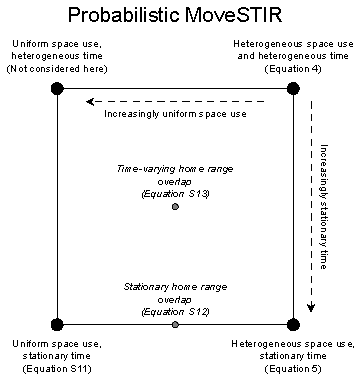
\includegraphics[width=\textwidth]{figures/conceptual_figure_pmovestir.pdf}
    \caption{Conceptual figure for PMoveSTIR}
\end{figure}

\end{document}
